\section{Measurement}
\label{sec:Measurement}

\subsection{Background measurement}

%Using two 30 X 30 X 2\cm wrapped plastic scintillators with photomultiplier tube (PMT) attached on iron test stand. 
%Each PMTs receives 1.5 kV high voltage and 350 V bias voltage. 
%Why do we set high voltage to 1.5 kV? Because rate increases with bigger high voltage, but it becomes flat when high voltage larger than 1.5 kV
%The scintillators measure mininum ionizing particles (mip).
%This supports by NIM crate.
%We test this equipments at lab taking cosimc rays
%This is the first time measured hit rate at underground cavern.
%Results from measurments may impact to other LLP experiments.
%When particle goes through scintillators and makes hits on both detectors, we counts number of events. 
%We made 30 mV threshold of signal pick to measure data which has physical meaning. 
%Triggering when signals appear at both detector in 5 ns. 
%Since detector have been placed 100 m below underground, muons from cosmic rays decay are suppressed. 
%We take data during MD and when the beam is online. 
%We switch the detector position several times. Also we take data while detector is rotated. 
%This is the first measurement of hit rate at D3 platform. 
%We use scope to take data, hit rate is not high. 
%We remotely connect to scope and able to manage scope.
%We took data from 4 different places. 
%Back of D3 platform of each corner and central position.
%Front D3 platform at central with parallel to beam line and make 45 degree with a beam line.

\subsection{Test-bench}
We used Herschel detector.
For PMT, model: R1828-01
Because, it has high anode current upper limit, wide range of gain variation, fast time response to fit in 25 ns, large entry window to increase light yield, good single electron separation.
The test-bench includes cosmic stand, scope with extended functions (auto save waveforms, coincidence logic), high voltage power supplies (1.5 kV, bias 350 V), current-voltage meter, laptop to remote connect to scope.

\begin{figure}[h]
\centering
    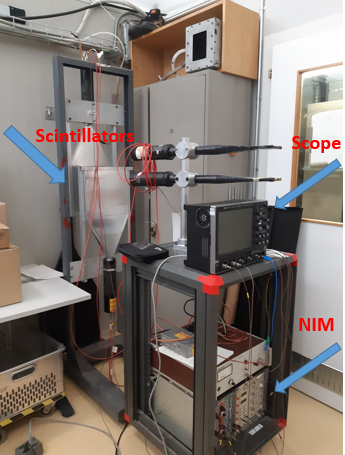
\includegraphics[width=5.5cm]{figs/INT/Tools.png} 
\caption{ 
    Test-bench photo
}
\end{figure}

\subsection{Trigger}
Simple 2x fold coincidence. 
Distance between two scintillators 2\cm. 
Discrimination (scope) threshold 30 mV.
When first scintillator receive a signal and the other scintillator also receives a signal in 5 ns, scope counts.
The scope automatically saved two waveforms from each scintillator and the number of mininum ionizing particles (mip) counted during the run.

\begin{figure}[h]
\centering
    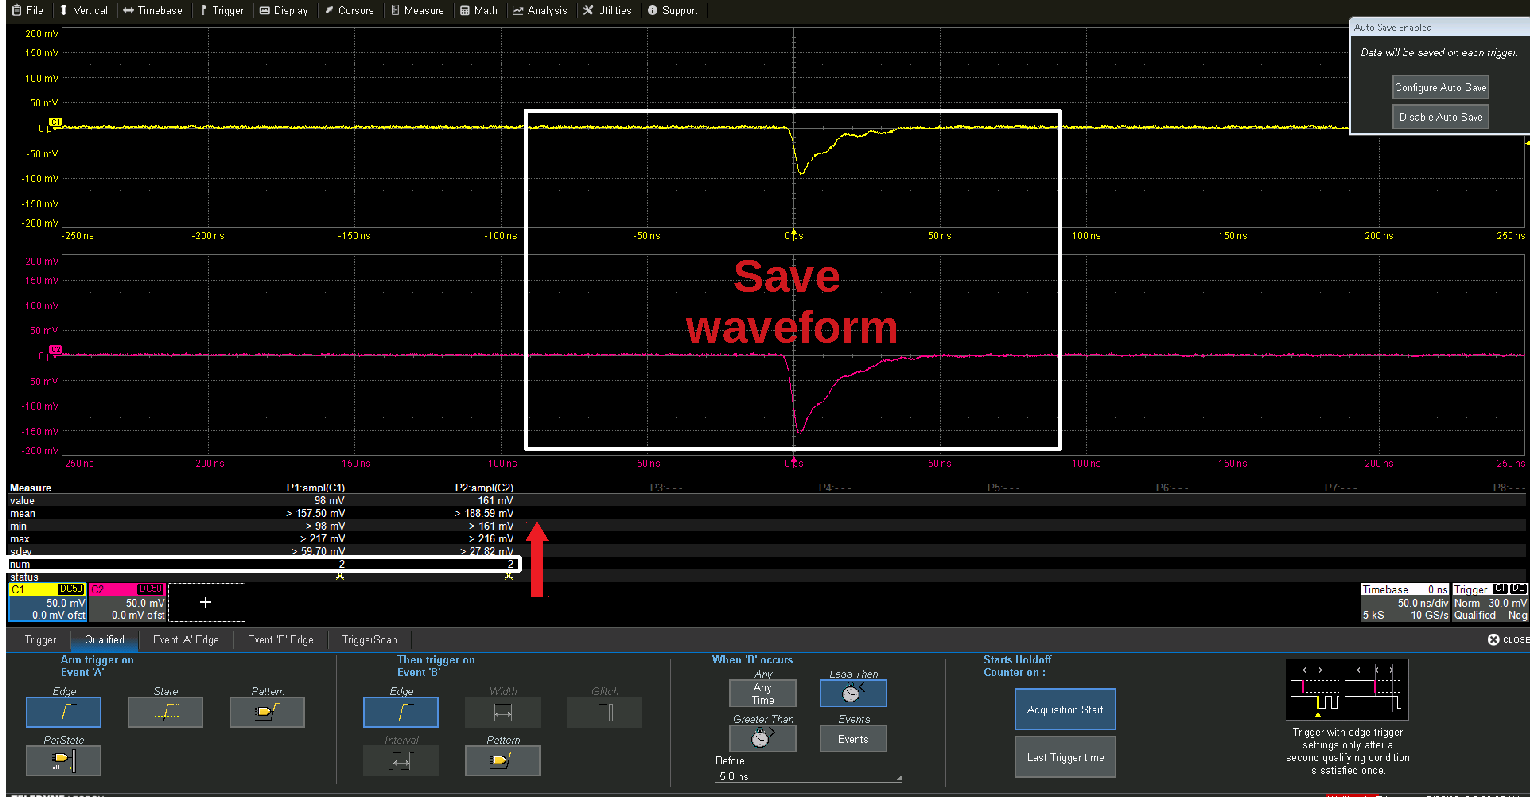
\includegraphics[width=16cm]{figs/INT/waveform.pdf}
\caption{
    Trigger setup using coincidence occurence of two signals in 5~ns. 
}
\end{figure}

\subsection{Detail Configuration}

The background measurement was taken at the LHCb cavern on D3 platform. The equipment had been set at 3 positions between DAQ racks and the concrete shield wall and the position between the \delphi and DAQ racks.
We basically placed the scintillator stand parallel to the beam line but also rotated $45^{\circ}$ and perpendicular to the beam line.
Fig 4. shows the positio

\begin{figure}[h]
\centering
    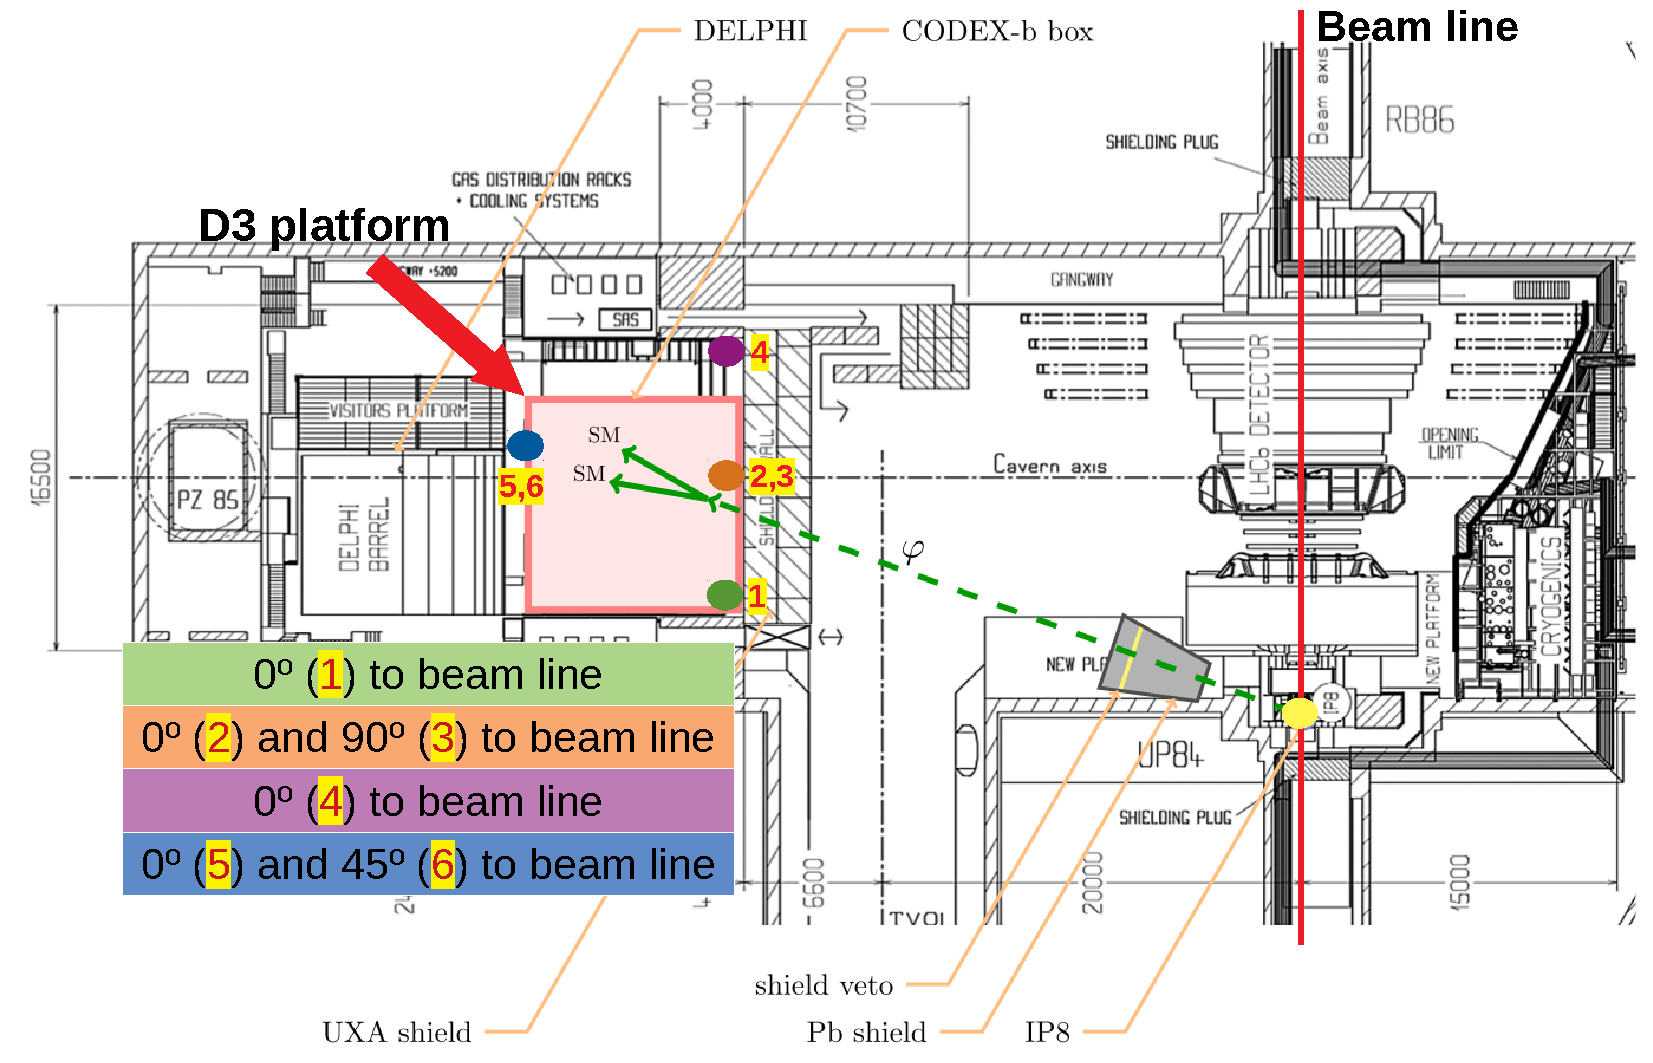
\includegraphics[width=16cm]{figs/INT/configuration.pdf}
\caption{
    Four measurement positions at the LHCb cavern
}
\end{figure}

\begin{figure}[h]
  \begin{center}
    \begin{tabular}[t]{cc}
      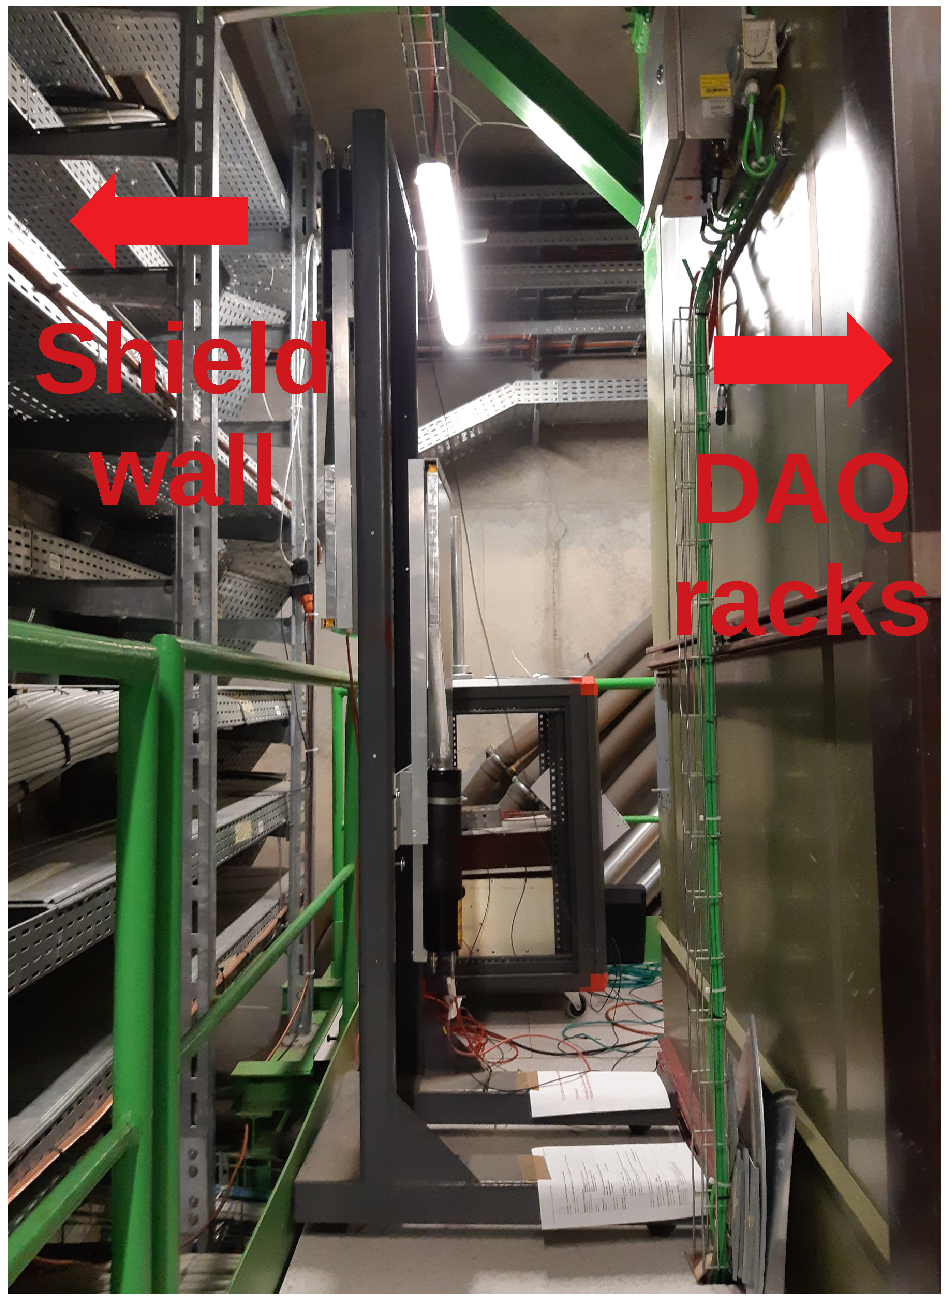
\includegraphics[width=0.5\textwidth]{figs/INT/Initial.pdf} &
      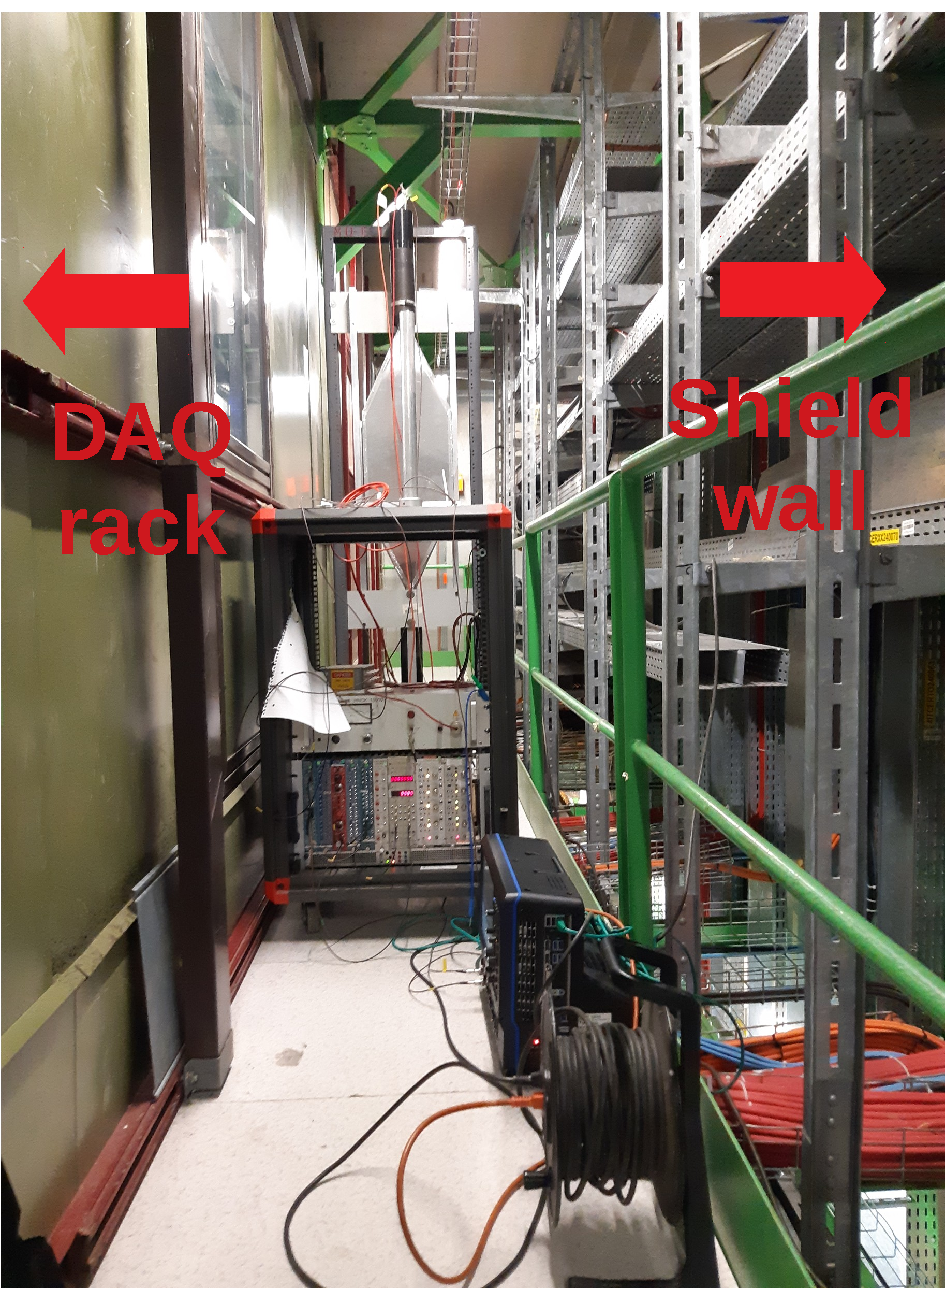
\includegraphics[width=0.5\textwidth]{figs/INT/Back_central.pdf} \\
      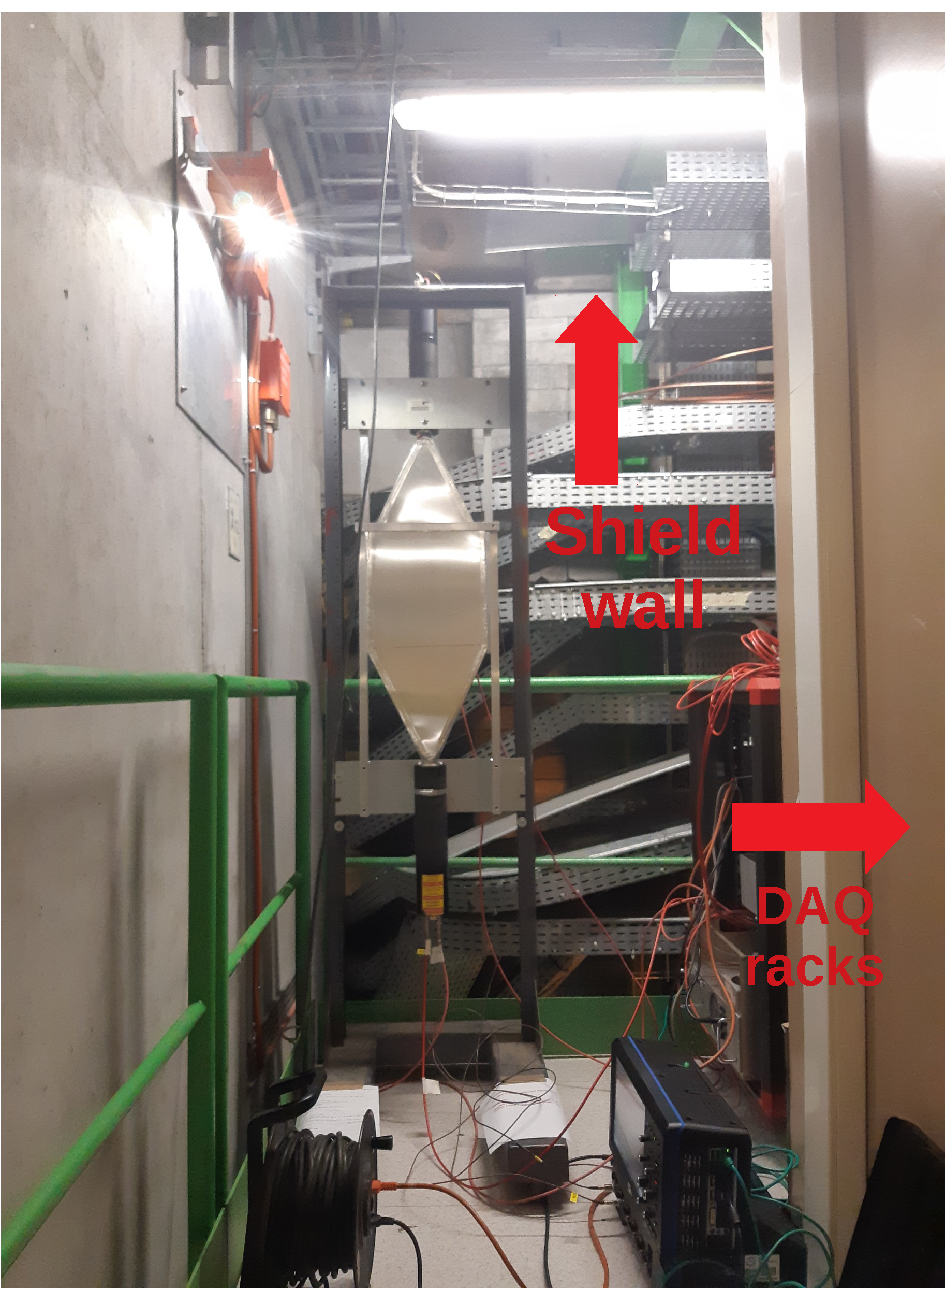
\includegraphics[width=0.5\textwidth]{figs/INT/Othercorner.pdf} &
      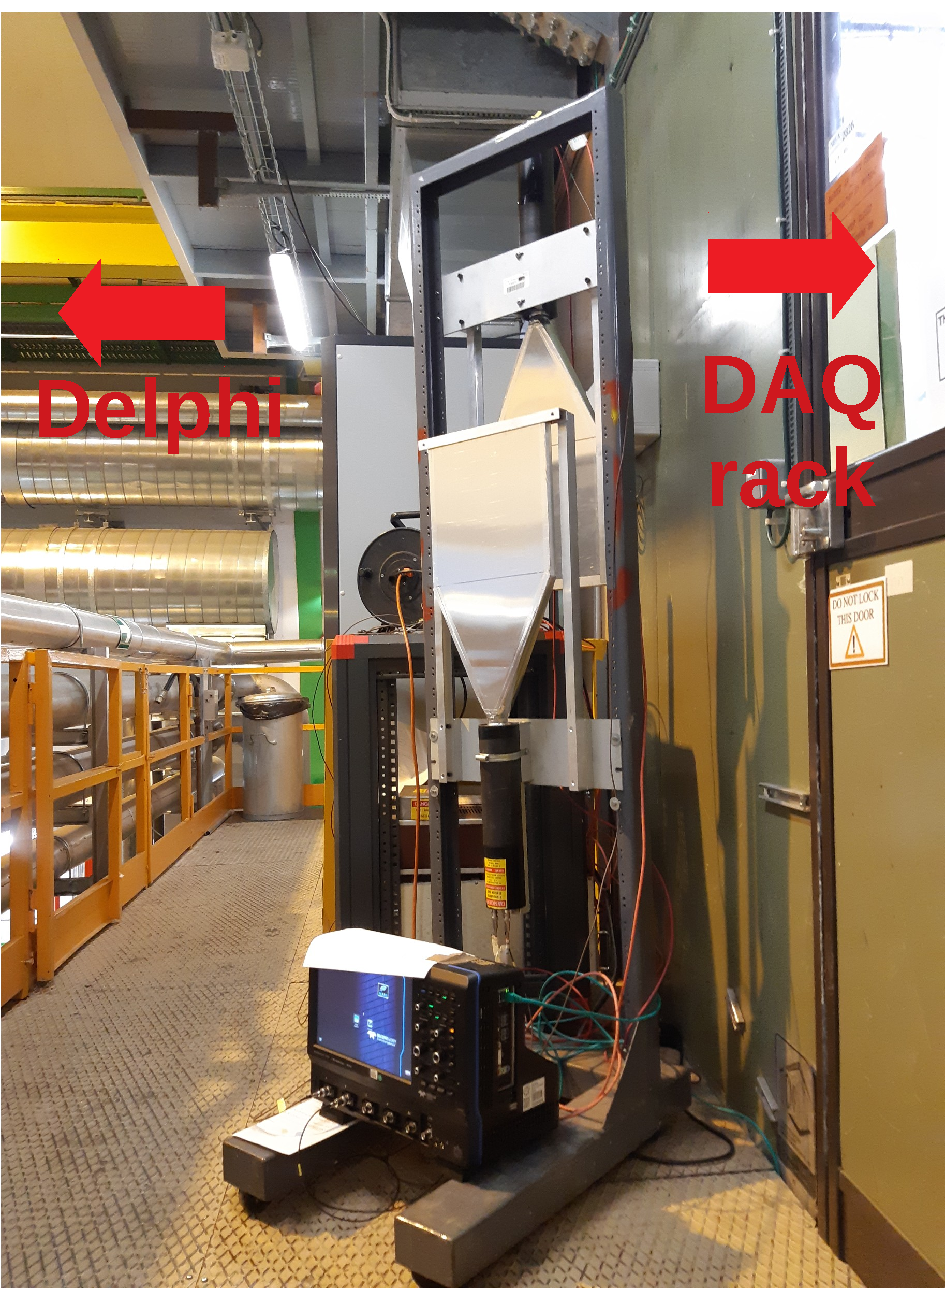
\includegraphics[width=0.5\textwidth]{figs/INT/D3_front.pdf} \\
    \end{tabular}
  \end{center}
\caption{
    Photos from each position
}
\end{figure}

\subsection{Results}

The measurement campagin spanning 17 days in July-Aug 2018.
The scope performed 52036 triggers during the run.

\begin{figure}[h]
\centering
    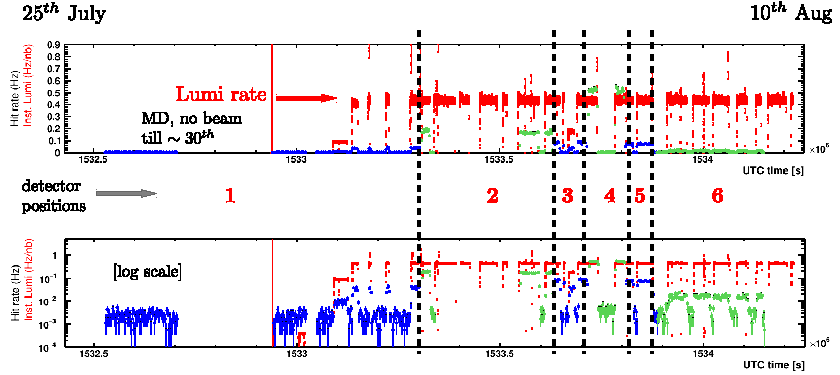
\includegraphics[width=14cm]{figs/INT/codexb_data_global.pdf}
\caption{
    Hit rate plots during the run based on 6 positions/configurations linear and log scale. Red dots mean the lumi rate of \lhcb, blue and green dots mean hit rates.
}
\end{figure}

\begin{center}
\begin{tabular}{c|l|r}
  Position & \hspace{2cm}Description & Hit rate [mHz] \\
  \hline \hline
   P1 & shield, right corner, $\parallel$ to beam& $1.99\pm0.07$ \\ \hline
   P2 & shield, center, $\parallel$ to beam&  $2.76\pm 0.03$ \\ \hline
   P3 & shield, center, $\perp$ to beam& $ 2.26\pm 0.03$ \\ \hline
   P4 & shield, left corner, $\parallel$ to beam& $ 3.11\pm 0.03$ \\ \hline
   P5 & shield + D3 racks, center, $\parallel$ to beam& $ 1.95\pm 0.03$ \\ \hline
   P6 & shield + D3 racks, center, $45^\circ$ to beam& $ 2.22\pm $ 0.02\\ \hline
\end{tabular}
\end{center}

\begin{center}
\begin{tabular}{c|l|r}
  Position & \hspace{0.9cm}Description & Hit rate [mHz] \\
  \hline \hline
   P1 & shield, right corner, $\parallel$ to beam & $ 38.99 \pm 0.99 $\\ \hline
   P2 & shield, center, $\parallel$ to beam& $ 167.10 \pm 1.43$ \\ \hline
   P3 & shield, center, $\perp$ to beam& $ 82.81 \pm 1.55 $ \\ \hline
   P4 & shield, left corner, $\parallel$ to beam& $ 517.45 \pm 3.52 $ \\ \hline
   P5 & shield + D3 racks, center, $\parallel$ to beam& $ 73.58 \pm 1.18 $ \\ \hline
   P6 & shield + D3 racks, center, $45^\circ$ to beam& $ 15.71 \pm 0.33 $ \\ \hline
\end{tabular}
\end{center}
